\chapter{Создание топологии} \label{chap:altium-PcbDoc}


\section{Создание и настройка правил}

Применённые стандартные правила приведены в следующем списке:
\begin{itemize}
	\item Зазор --- 0.15 мм
	\item Защита от КЗ
	\item Запрет на свободные и висящие концы и пины.
	\item Ширина
		\begin{itemize}
			\item ВЧ линий: 0.2-1.1-1.15~мм
			\item Остальных линий: 0.2-0.3-0.5~мм
		\end{itemize}
	\item ВЧ углы скругляются с двух сторон, остальные срезаются.
	\item Переходные отверстия 0.8х0.4~мм
	\item Зазор  от металлизации  до  выреза паяльной маски 0.05~мм
	\item Расстояние от полигона до элемента 0.2~мм
	\item Угол минимум  60°  для  всех видов металлизированных примитивов. 
	\item Отверстия от 0.4 до 3.5~мм с минимальным шагом в 0.2~мм
	\item Минимальный мостик паяльной маски --- 0.125~мм
	\item Зазор 0.15~мм для шелкографии
	\item Установим расстояние в 0.25~мм от края платы до любого элемента, кроме полигонов --- для торцевой металлизации зазор между платой и полигоном должен быть равен 0.
	\item Минимальные зазоры для 3D моделей --- 0.2~мм по Ox и 0.1~мм по Oy
\end{itemize}

Конфигурация слоёв платы остаётся такой же как и у посадочных мест.

Цветовая схема - "Неважно какого цвета ваша плата, главное чтобы синяя!".

\section{Разводка печатной платы}
Есть два способа расположить элементы:
\begin{itemize}
	\item С одной стороны ВЧ тракта на однослойной плате;
	\item По разные стороны, но плата потребуется многослойная.
\end{itemize}
Рассмотрим оба варианта.

\begin{figure}[H]
	\centering\
	\begin{subfigure}[b]{\textwidth}
		\centering
		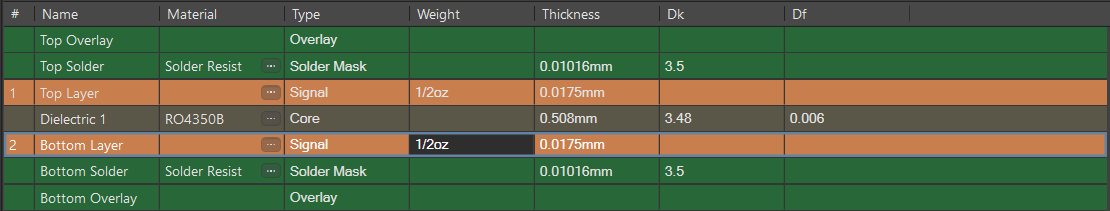
\includegraphics[width=\textwidth]{2LayerStackup.png}
		\caption{}%
		\label{fig:2LayerStackup}
	\end{subfigure}
	\hfill
	\begin{subfigure}[b]{\textwidth}
		\centering
		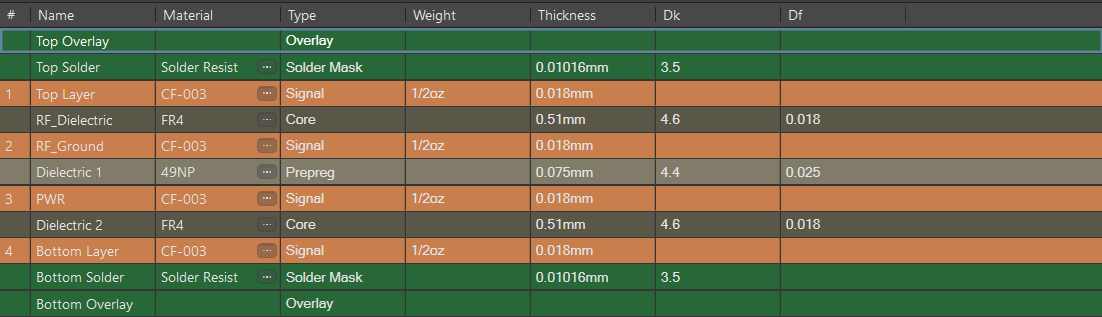
\includegraphics[width=\textwidth]{4LayerStackup.png}
		\caption{}%
		\label{fig:4LayerStackup}
	\end{subfigure}
	\caption{%
		Stackup платы
		(а) двухслойной;
		(б) четырёхслойной
	}%
	\label{fig:Stackup}
\end{figure}

В обоих вариантах потребуется создать вырез в заливке для ВЧ линии, чтобы учитывать её размеры создадим набросок границы полигона используя инструмент Poligon Pour Cutout. (Рис. \ref{fig:DraftPolyCut})

Элементы будем располагать так, чтобы различные фильтры, стабилизаторы и т.д. располагались максимально близко к месту применения. Также дополнительно добавим символику университета на свободное место.

\begin{figure}[H]
	\centering
	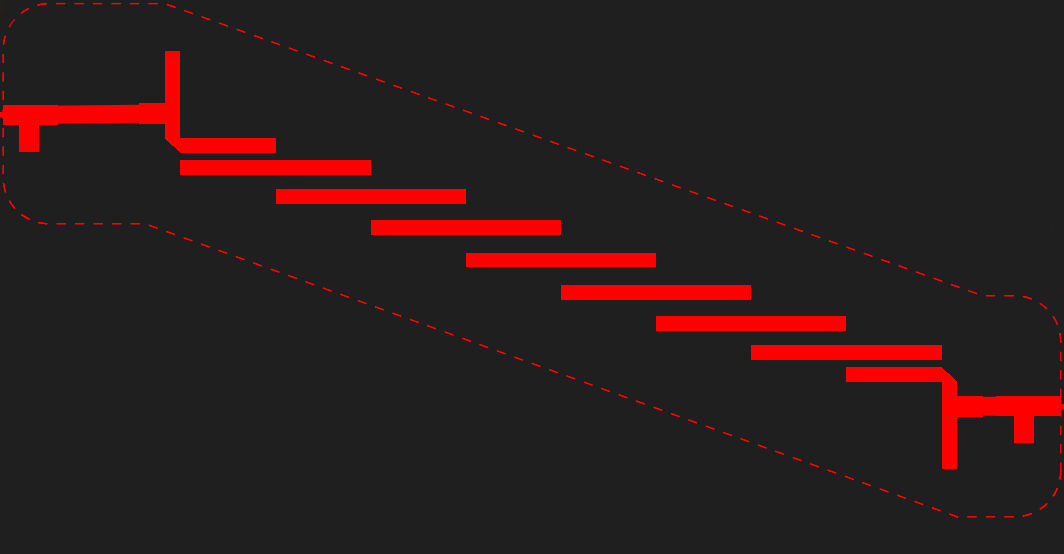
\includegraphics[width=0.8\textwidth]{DraftPolyCut.png}
	\caption{Вырез в заливке.}%
	\label{fig:DraftPolyCut}
\end{figure}

Послойный вид двухслойной платы можно увидеть на Рис. \ref{fig:2LayerPCB}

\begin{figure}[H]
	\centering\
	\begin{subfigure}[b]{0.45\textwidth}
		\centering
		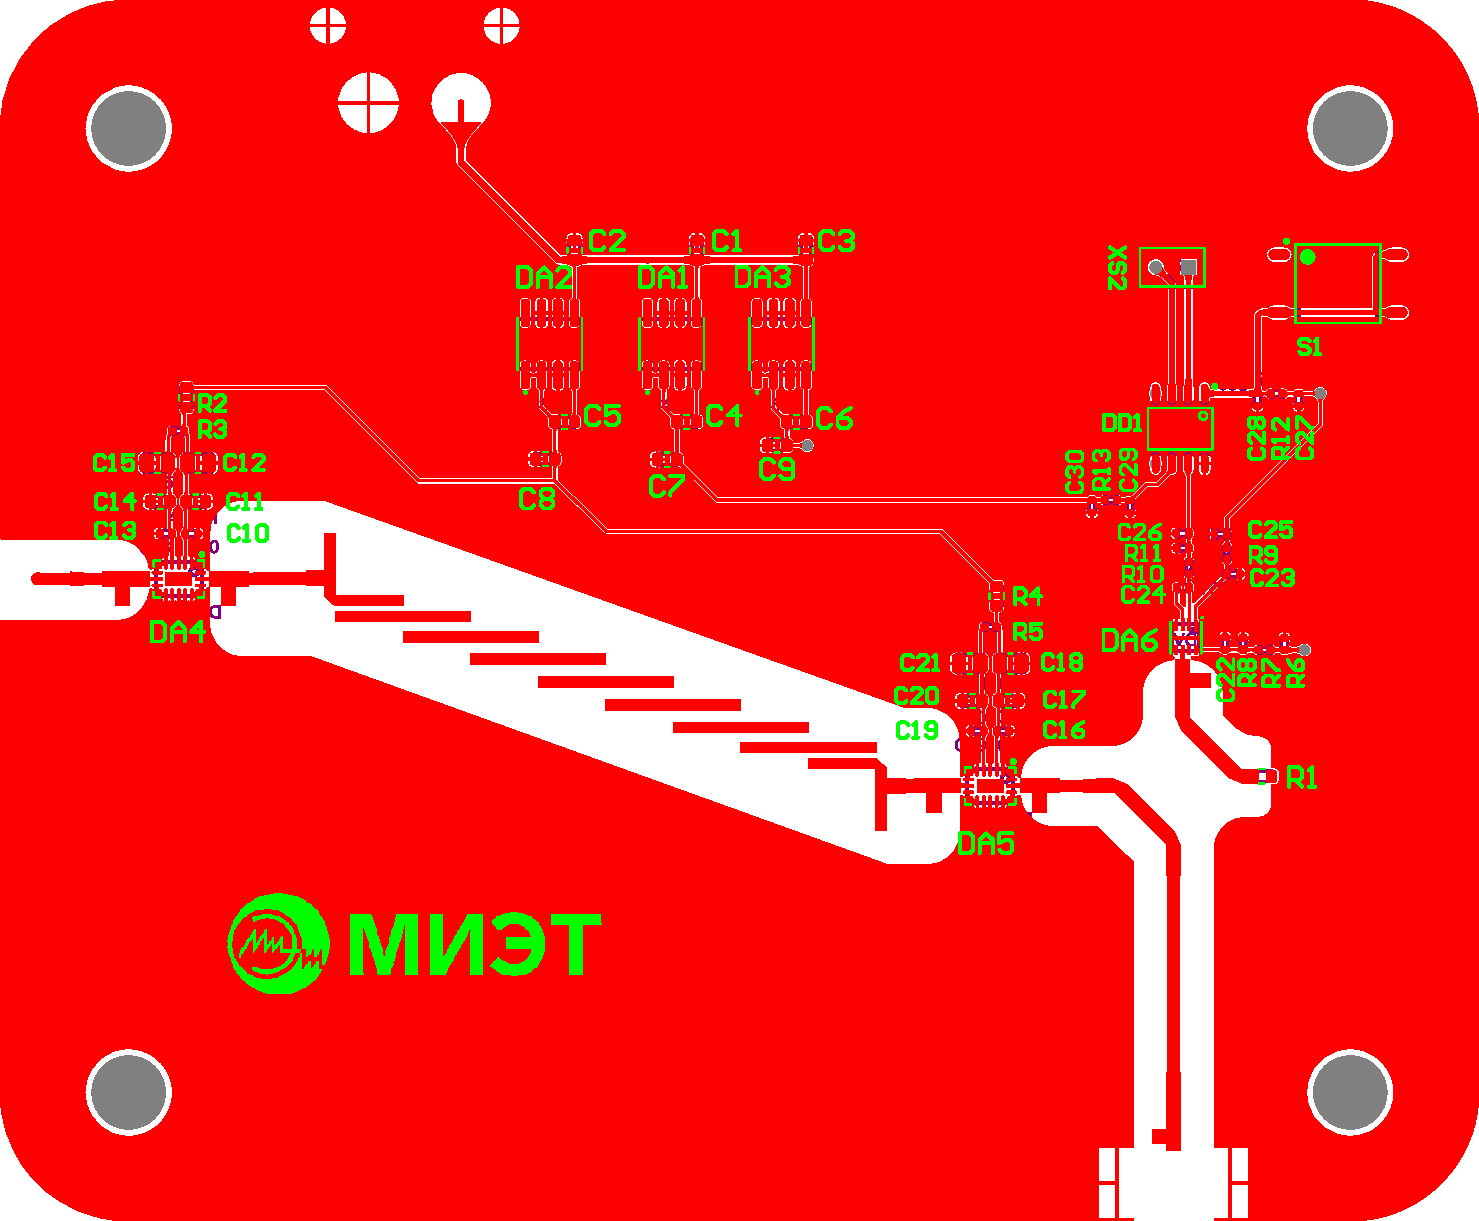
\includegraphics[width=\textwidth]{2LayerTL.pdf}
		\caption{}%
		\label{fig:2LayerTL}
	\end{subfigure}
	\hfill
	\begin{subfigure}[b]{0.45\textwidth}
		\centering
		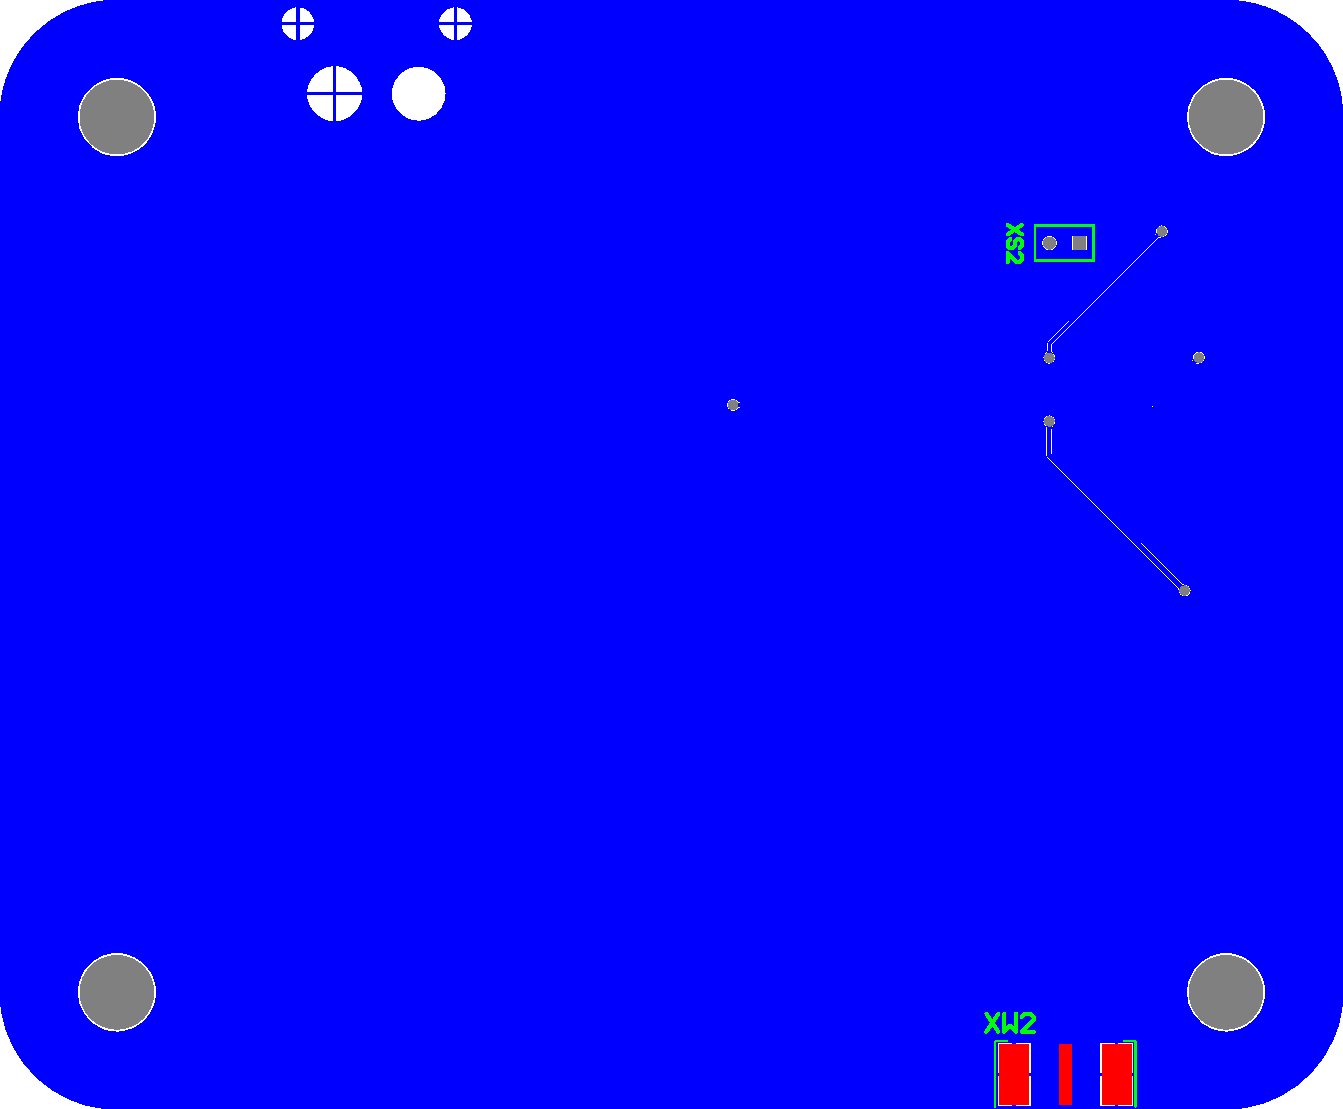
\includegraphics[width=\textwidth]{2LayerBL.pdf}
		\caption{}%
		\label{fig:2LayerBL}
	\end{subfigure}
	\caption{%
		Разводка двухслойной платы
		(а) Верхний слой;
		(б) Нижний слой
	}%
	\label{fig:2LayerPCB}
\end{figure}
 Для улучшения ВЧ свойств платы прошьём её используя инструмент Via Snitching to Net. (Рис. \ref{fig:2LayerAll}) и вскроем маску для ВЧ линий.
 \begin{figure}[H]
 	\centering
 	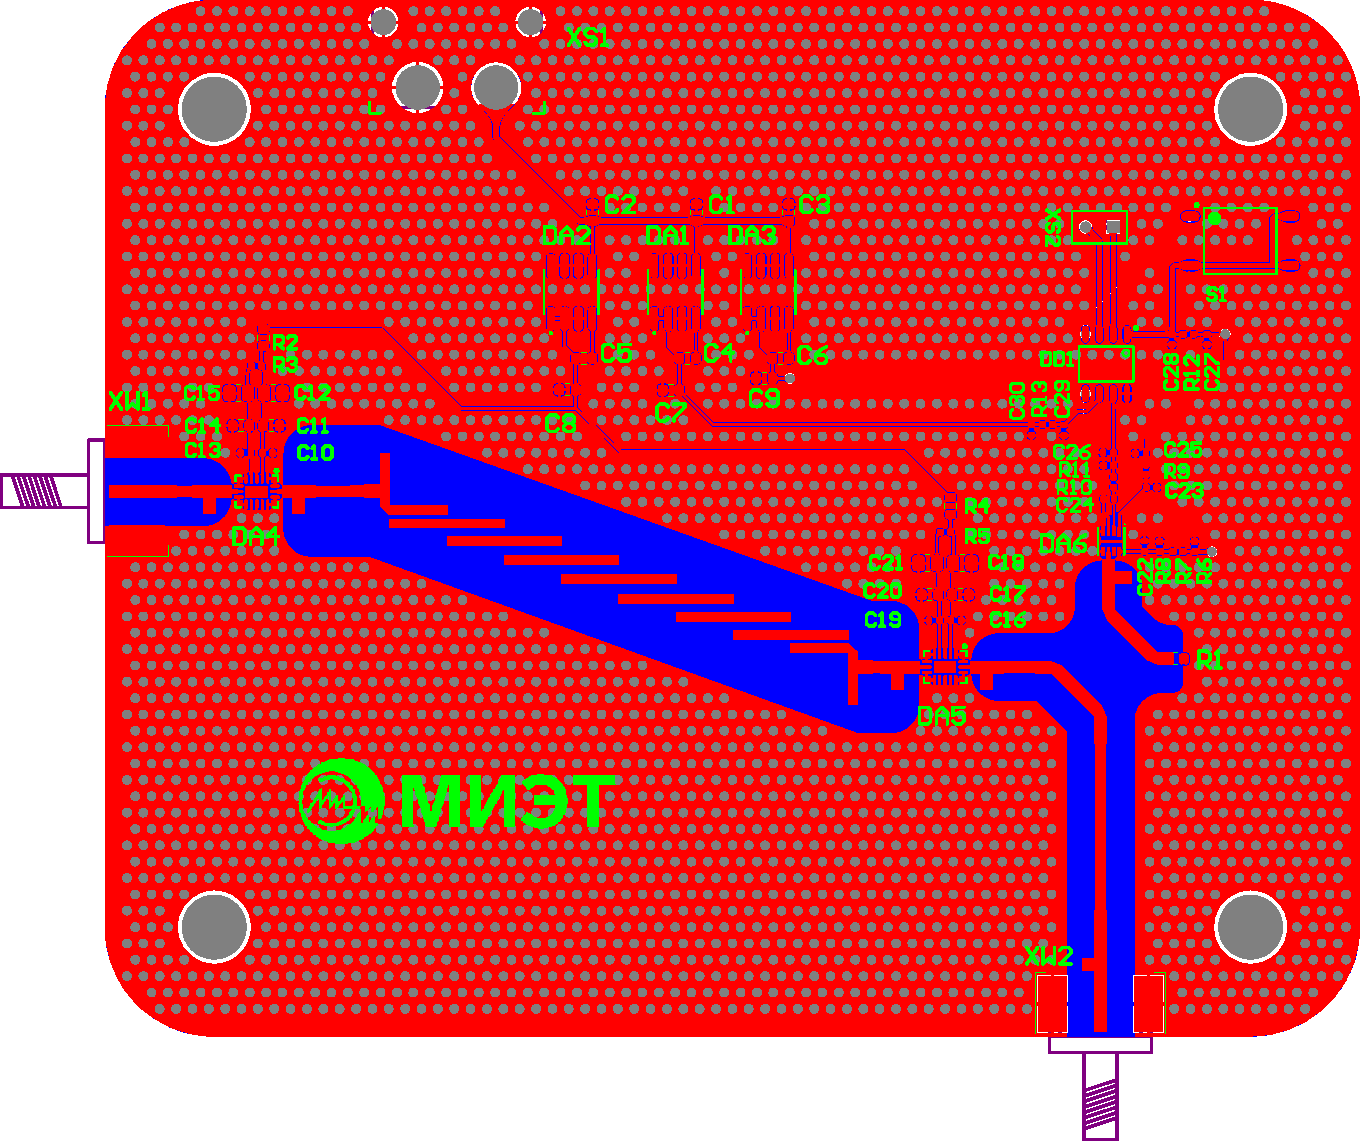
\includegraphics[width=0.45\textwidth]{2LayerAll.pdf}
 	\caption{Конечный вариант.}%
 	\label{fig:2LayerAll}
 \end{figure}

Послойный вид четырёхслойной платы можно увидеть на Рис. \ref{fig:4LayerPCB}

\begin{figure}[H]
	\centering\
	\begin{subfigure}[b]{0.45\textwidth}
		\centering
		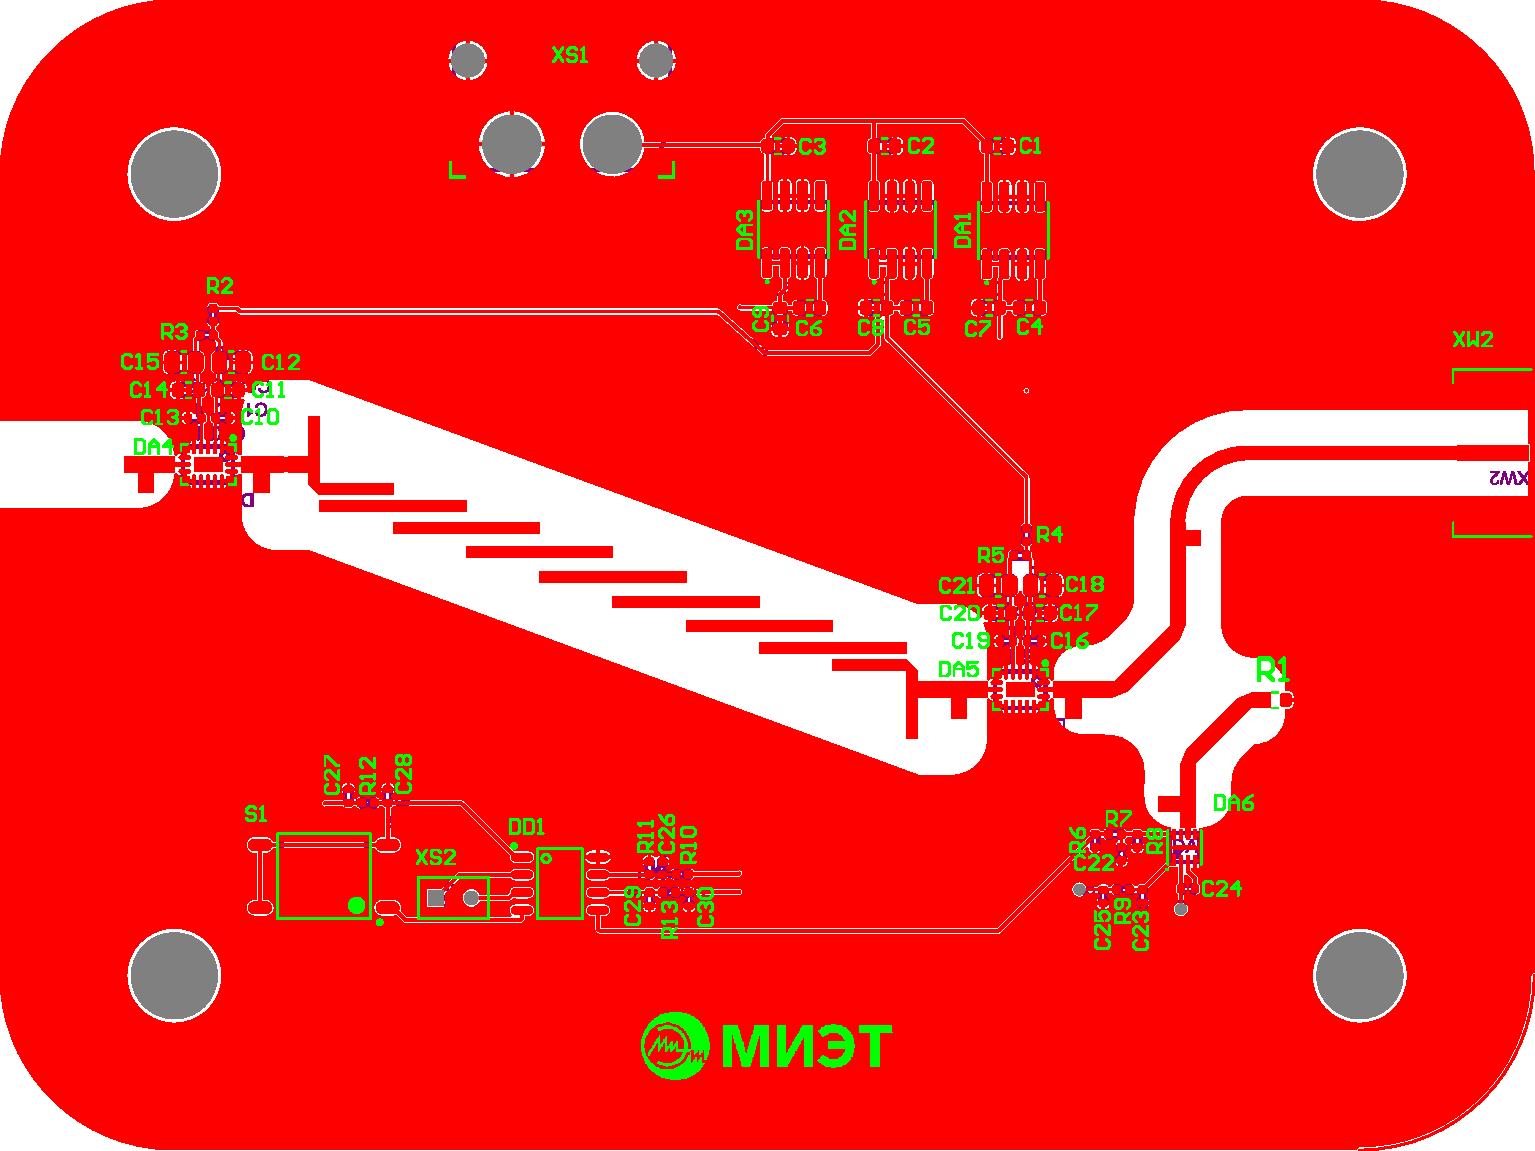
\includegraphics[width=\textwidth]{4LayerTL.pdf}
		\caption{}%
		\label{fig:4LayerTL}
	\end{subfigure}
	\hfill
	\begin{subfigure}[b]{0.45\textwidth}
		\centering
		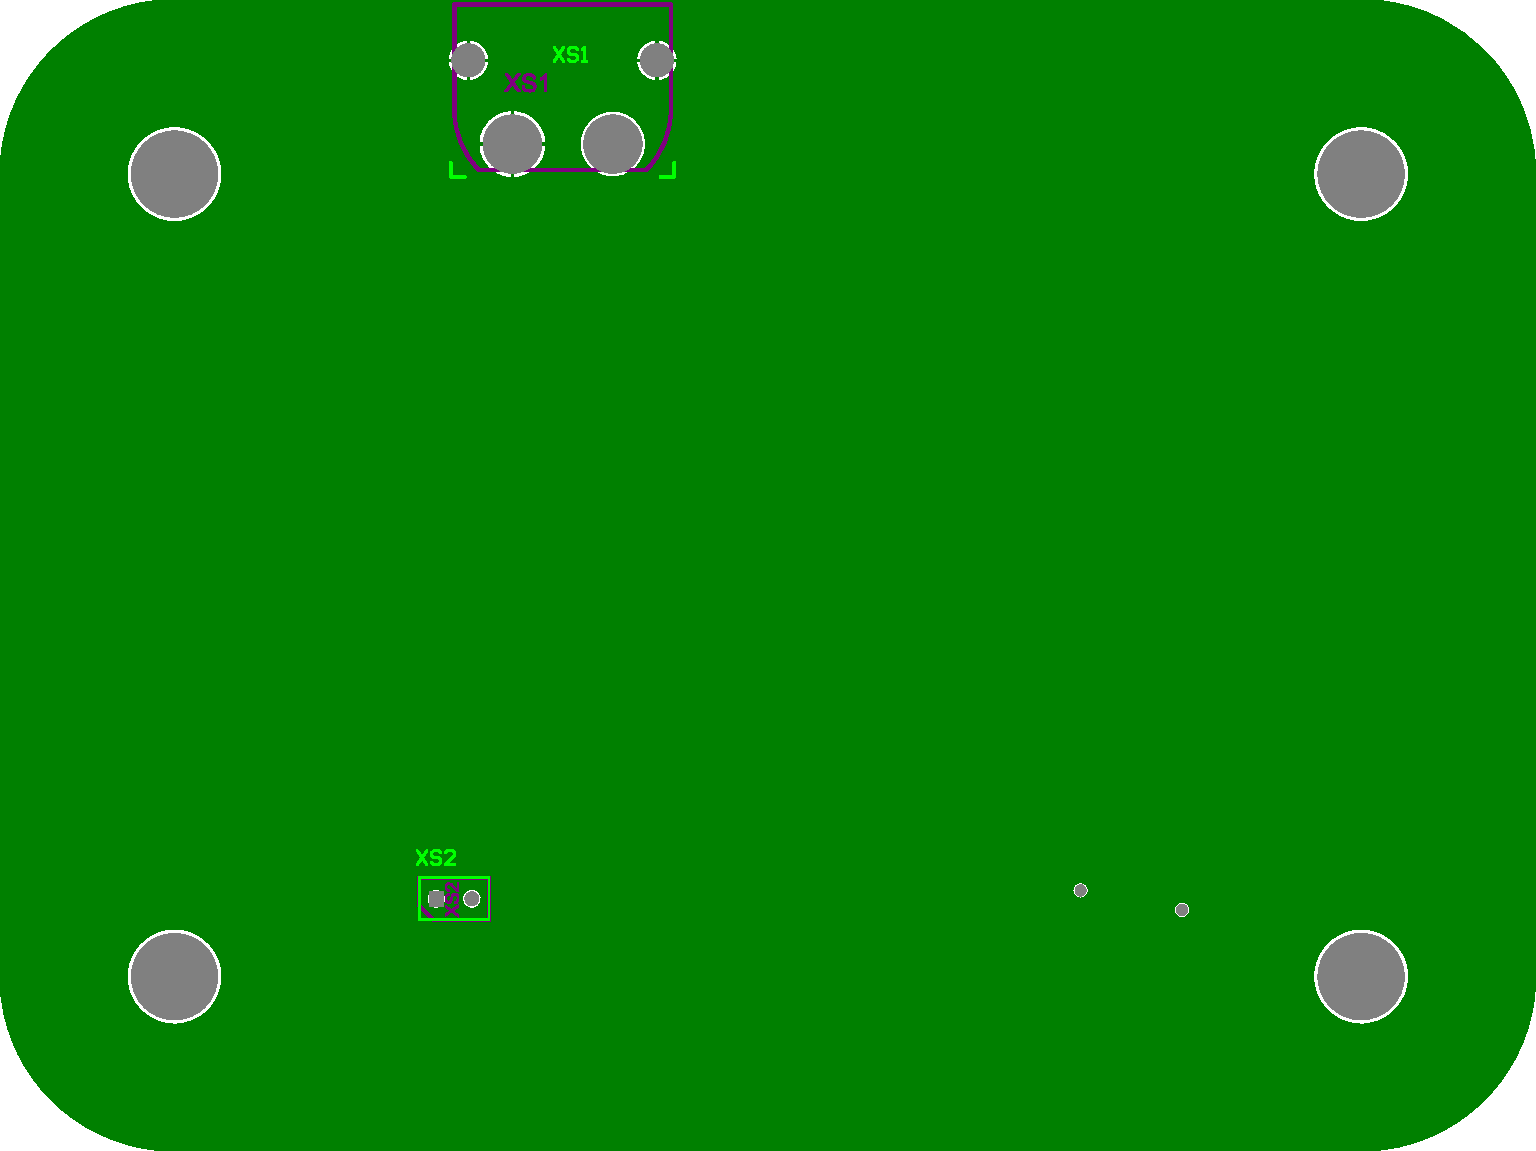
\includegraphics[width=\textwidth]{4LayerRF.pdf}
		\caption{}%
		\label{fig:4LayerRF}
	\end{subfigure}
	\hfill
	\begin{subfigure}[b]{0.45\textwidth}
		\centering
		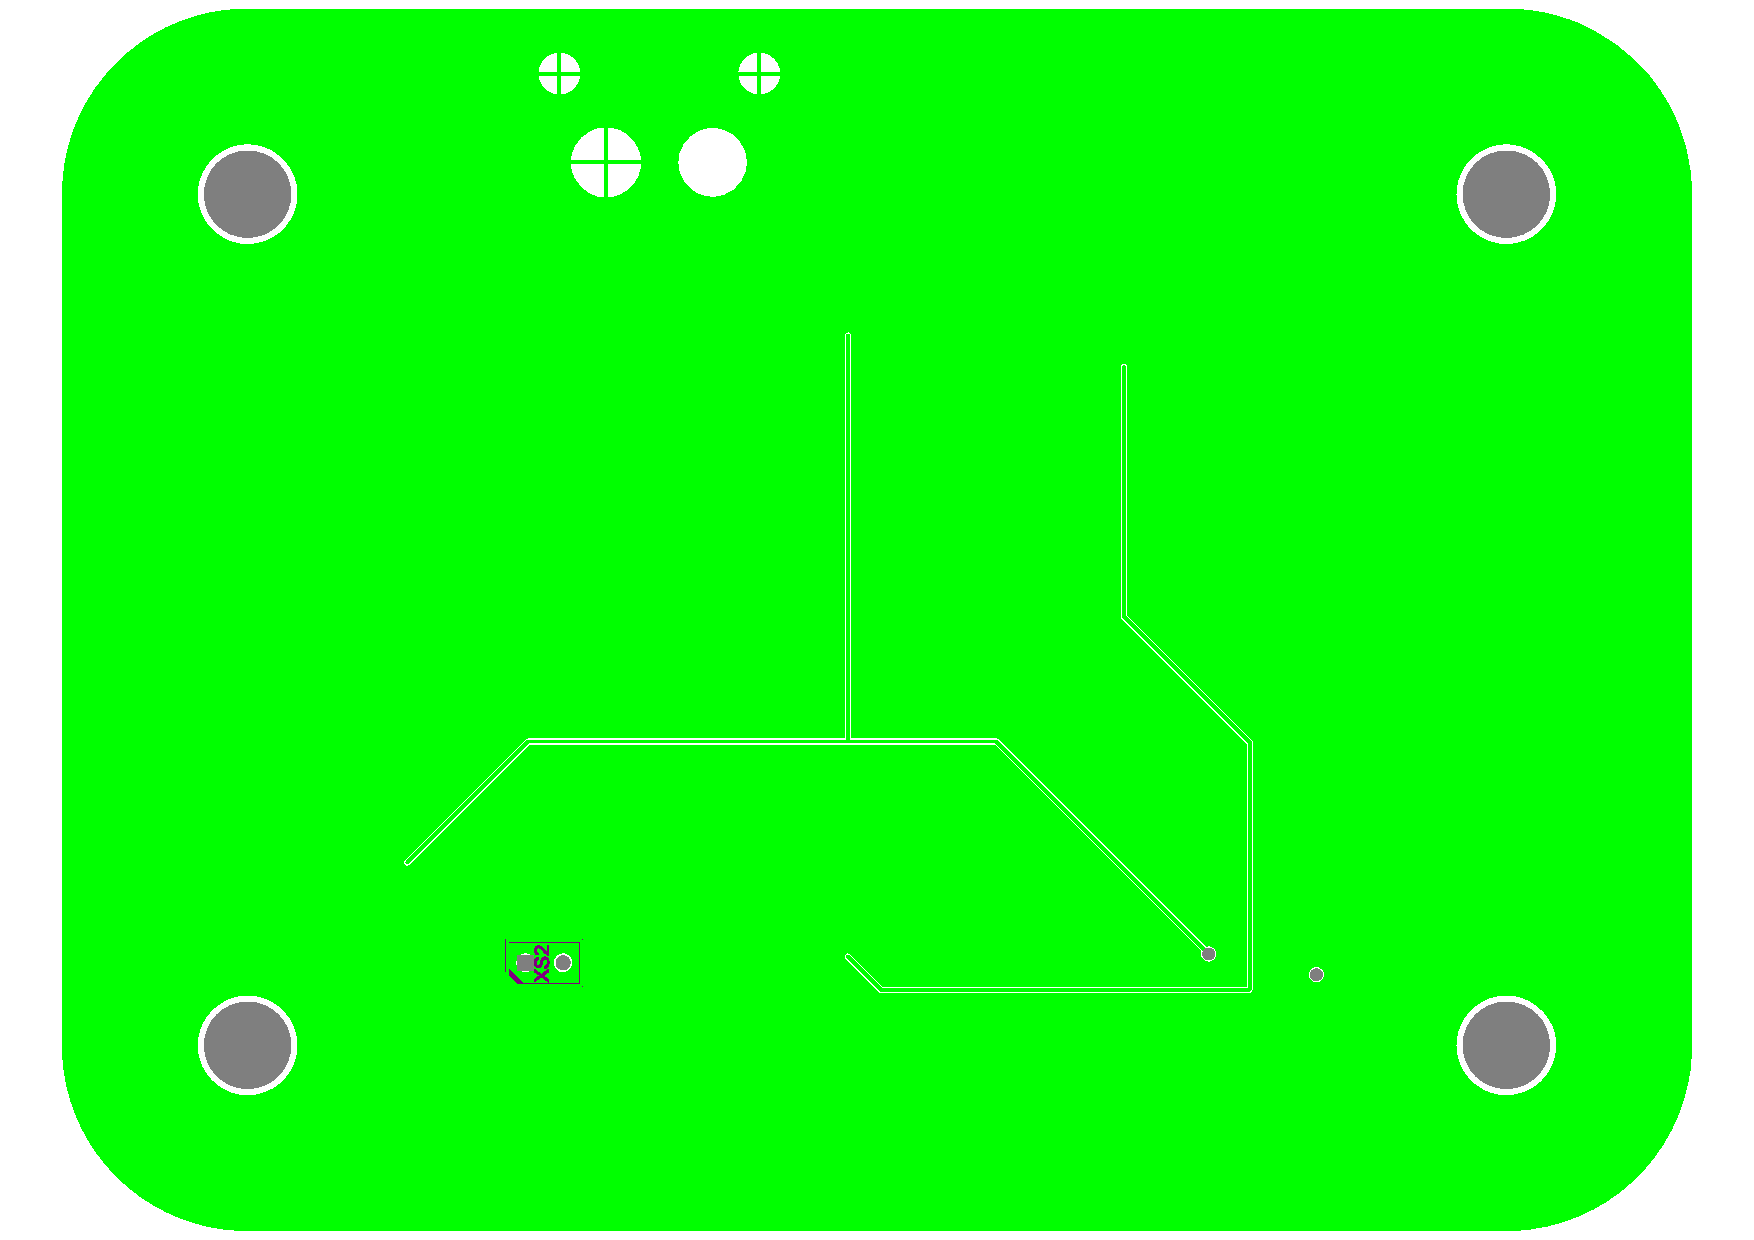
\includegraphics[width=\textwidth]{4LayerPWRL.pdf}
		\caption{}%
		\label{fig:4LayerPWRL}
	\end{subfigure}
	\hfill
	\begin{subfigure}[b]{0.45\textwidth}
		\centering
		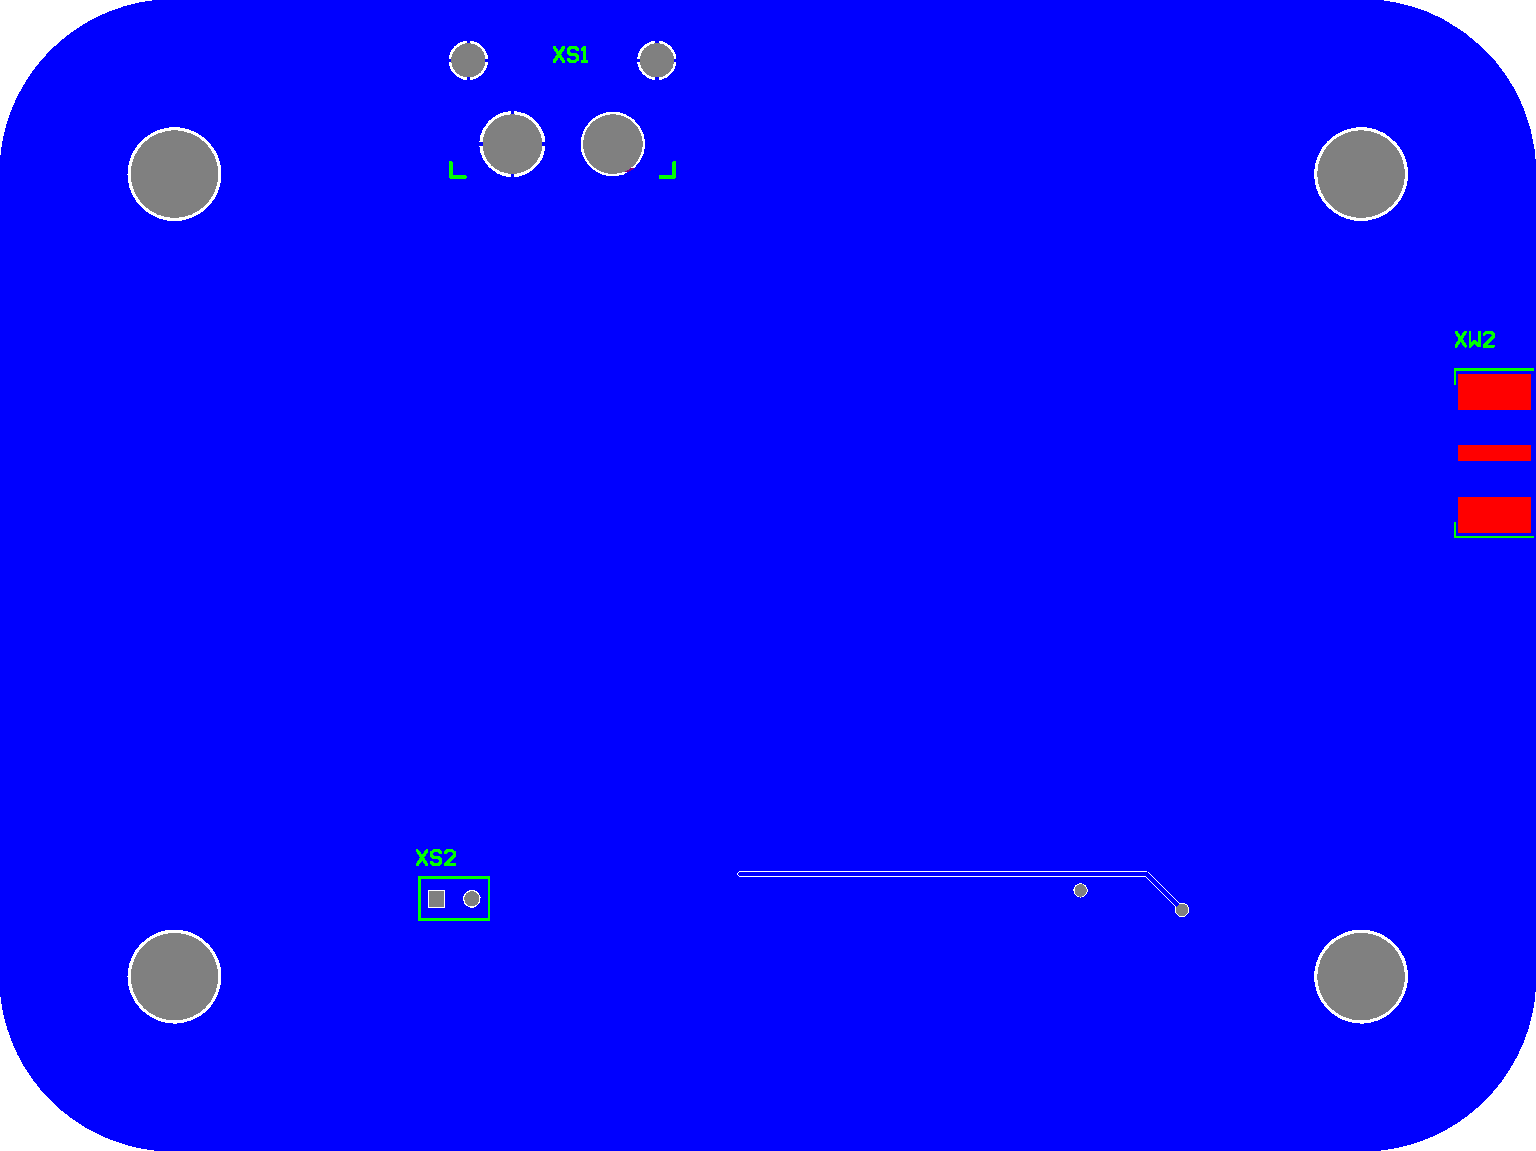
\includegraphics[width=\textwidth]{4LayerBL.pdf}
		\caption{}%
		\label{fig:4LayerBL}
\end{subfigure}
	\caption{%
		Разводка четырёхслойной платы
		(а) Верхний слой;
		(б) ВЧ земля;
		(в) PWR-слой;
		(г) Нижний слой.
	}%
	\label{fig:4LayerPCB}
\end{figure}
Для улучшения ВЧ свойств платы прошьём её используя инструмент Via Snitching to Net. (Рис. \ref{fig:4LayerAll}) и вскроем маску для ВЧ линий.
\begin{figure}[H]
	\centering
	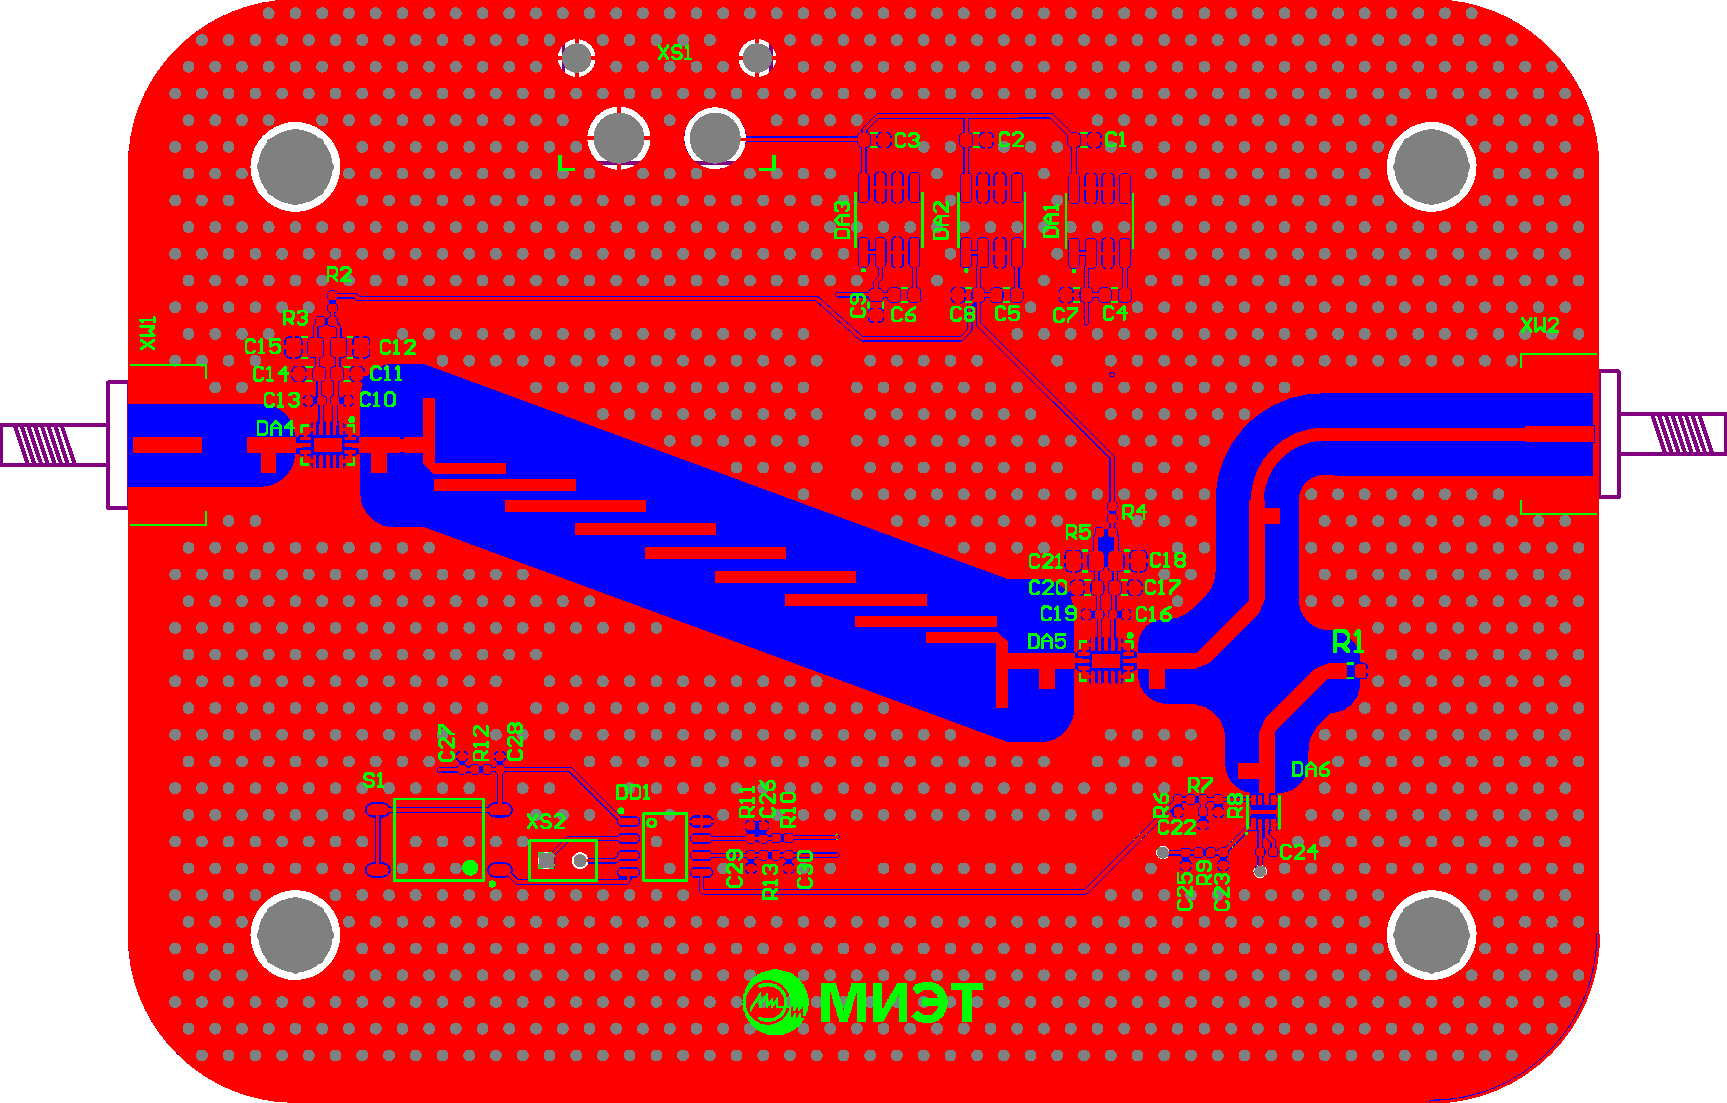
\includegraphics[width=0.7\textwidth]{4LayerAll.pdf}
	\caption{Конечный вариант.}%
	\label{fig:4LayerAll}
\end{figure}

\section{Итоговый вид}

\begin{figure}[H]
	\centering\
	\begin{subfigure}[b]{0.45\textwidth}
		\centering
		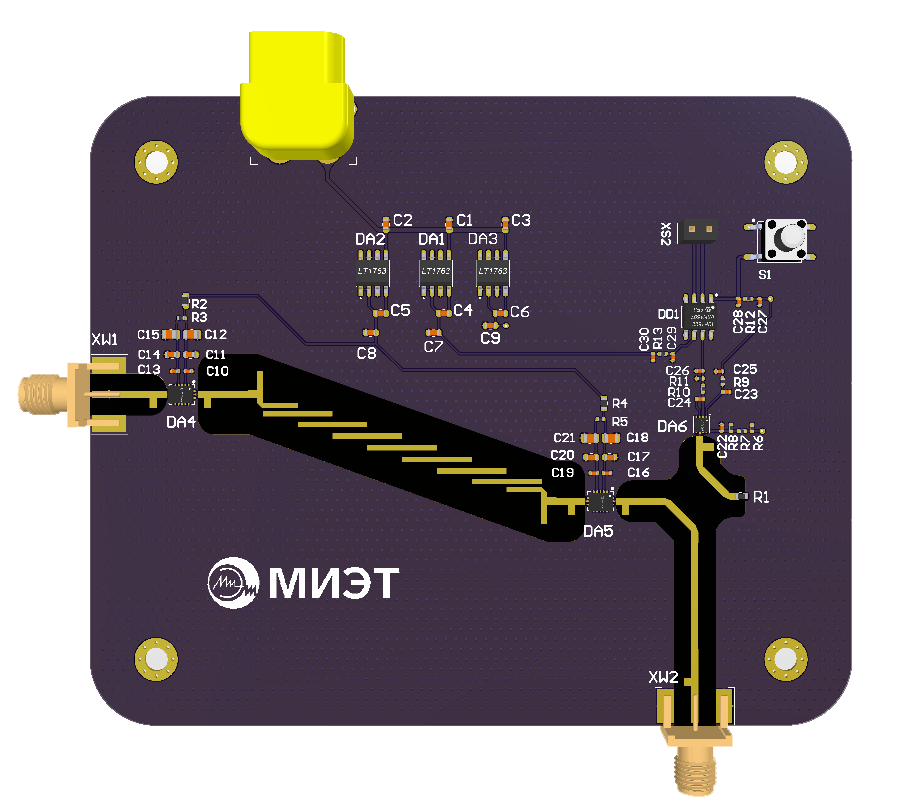
\includegraphics[width=0.8\textwidth]{2Layer1.png}
		\caption{}%
		\label{fig:2Layer1}
	\end{subfigure}
	\hfill
	\begin{subfigure}[b]{0.45\textwidth}
		\centering
		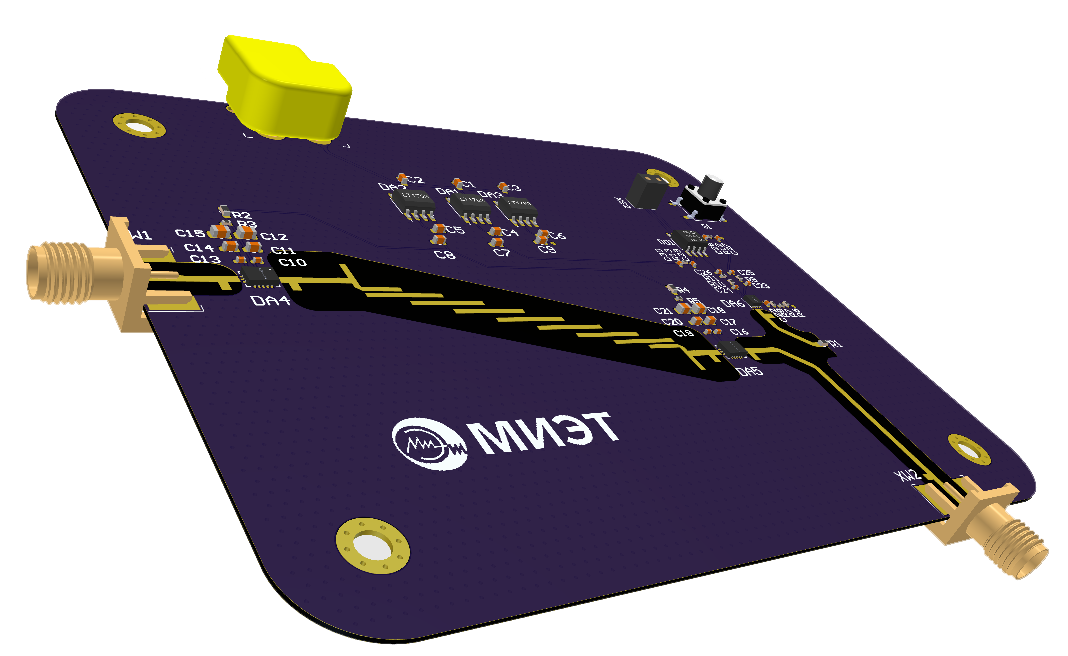
\includegraphics[width=\textwidth]{2Layer0.png}
		\caption{}%
		\label{fig:2Layer0}
	\end{subfigure}
	\caption{%
		Вид двухслойной платы:
		(а) Главный;
		(б) Изометрический.
	}%
	\label{fig:2Layer3D}
\end{figure}

\begin{figure}[H]
	\centering\
	\begin{subfigure}[b]{0.45\textwidth}
		\centering
		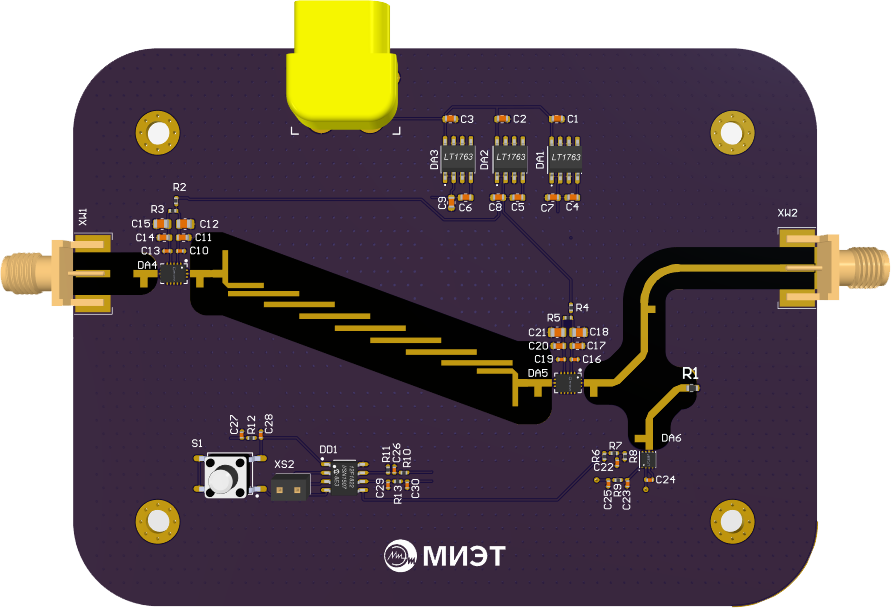
\includegraphics[width=\textwidth]{4Layer1.png}
		\caption{}%
		\label{fig:4Layer1}
	\end{subfigure}
	\hfill
	\begin{subfigure}[b]{0.45\textwidth}
		\centering
		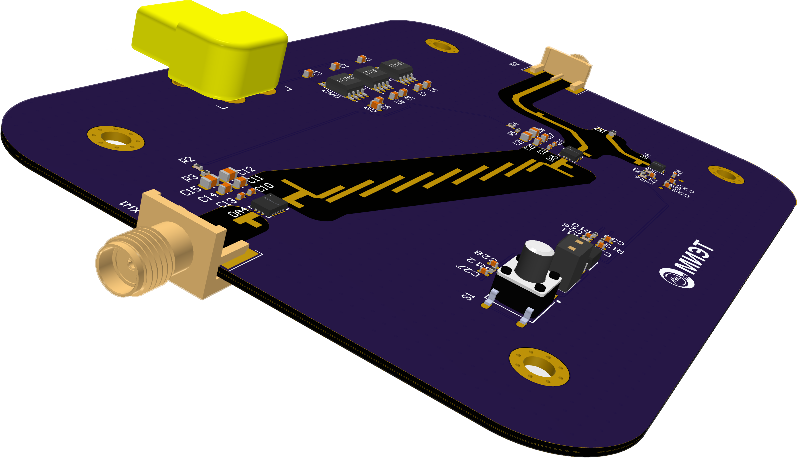
\includegraphics[width=\textwidth]{4Layer0.png}
		\caption{}%
		\label{fig:4Layer0}
	\end{subfigure}
	\caption{%
		Вид четырёхслойной платы:
		(а) Главный;
		(б) Изометрический.
	}%
	\label{fig:4Layer3D}
\end{figure}

Размеры плат:
\begin{itemize}
	\item Двухслойной: 115x95~мм;
	\item Четырёхслойной: 110x82.5~мм.
\end{itemize}

Ввиду приблизительно равных размеров плат дальнейшее проектирование будет проводиться только для двухслойной платы.